\documentclass[12pt, a4 paper]{article}
% Set target color model to RGB
\usepackage[inner=2.0cm,outer=2.0cm,top=2.5cm,bottom=2.5cm]{geometry}
\usepackage{setspace}
\usepackage[rgb]{xcolor}
\usepackage{verbatim}
\usepackage{subcaption}
\usepackage{outlines}
\usepackage{amsgen,amsmath,amstext,amsbsy,amsopn,tikz,amssymb,tkz-linknodes}
\usepackage{fancyhdr}
\usepackage{pgfplots}
\usepackage[colorlinks=true, urlcolor=blue,  linkcolor=blue, citecolor=blue]{hyperref}
\usepackage[colorinlistoftodos]{todonotes}
\usepackage{rotating}
\usepackage{graphicx}
\usepackage{enumitem}

\setlist[enumerate,1]{label=\textbf{\arabic*}}
\setlist[enumerate,2]{label=\textbf{\alph*})}
\setlist[enumerate,3]{label=\textbf{\roman*})}
\setlist{nosep}
\linespread{1.6} % Double Line Spacing

\graphicspath{ {./img/} }
\usepgfplotslibrary{fillbetween}

\hypersetup{%
pdfauthor={Vignesh Ravibaskar},%
pdfcreator={PDFLaTeX},%
pdfproducer={PDFLaTeX},%
}

\title{Vectors}
\author{Derek, Vignesh}
\date{2020}

\begin{document}

\maketitle
\textbf{VECTORS [150 Marks]}
\begin{outline}[enumerate]
	\1 Solve the following:
	\2 $\overrightarrow {OA}  = {\bf{a}}$ and $\overrightarrow {OB}  = {\bf{b}}$, where $O$ is the origin. Given that lines $OA$ and $OB$ are parallel, $\left| {\bf{a}} \right| = 2$ and ${\bf{a}} \cdot {\bf{b}} =  - 2$, express $\bf{b}$ in terms of $\bf{a}$.\hfill[2]

	\2 A vector \textbf{a} is such that ${\bf{a}} = (\sqrt 2 \cos \alpha ){\bf{i}} - (\cos \alpha ){\bf{j}} + (\sqrt 2 \sin \alpha ){\bf{k}}$, where $0 \le \alpha  \le 2\pi $ and $\left| {\bf{a}} \right| = \sqrt 2 $. Find the value(s) of $\alpha $.\hfill[2]

	\2 The points $A, B$ and $C$ with respect to the origin are represented by the vectors ${\bf{a}}$, ${\bf{b}}$ and ${\bf{c}}$ respectively. It is given that $\left| {\bf{b}} \right| = 2$, ${\bf{a}} \cdot {\bf{b}} = k$ and ${\bf{b}} \cdot {\bf{c}} = 2$. Given further that point $C$ divides the line $AB$ such that $AC:CB = 2:1$, find $k$.\hfill[3]

	\2 Four vectors \textbf{a}, \textbf{b}, \textbf{c} and \textbf{d} exist such that ${\bf{a}} + {\bf{b}} + {\bf{c}} + {\bf{d}} = {\bf{0}}$. Show that ${\bf{b}} \times ({\bf{a}} + {\bf{c}}) = {\bf{d}} \times {\bf{b}}$.\hfill[2]

	\2 Point $A$ referred from the origin has vector ${\bf{a}} = {\bf{i}} + 2{\bf{j}} - 2{\bf{k}}$. The line $OA$ makes an angle of $\alpha $ with the $y$-axis and $\beta $ with the $z$-axis, where $\alpha ,\beta  < \pi $. Show that $\alpha  + \beta  = \pi $.\hfill[3]\\

	\1 Referred to the origin $O$, points $A$ and $B$ have position vectors given by ${\bf{a}}$ and ${\bf{b}}$ respectively. ${C_0}$ is the foot of perpendicular from $A$ to $OB$ with position vector ${{\bf{c}}_0}$. The angle between lines $OA$ and $OB$ is $\alpha$ , where $ 0< \alpha  < \dfrac{\pi}{2}$.

	\2 By considering $\cos{\alpha}$, show that $|{\bf{c}}_0|= {\bf{a}} \cdot {\bf{\hat b}}$.\hfill[2]

	\2 The foot of perpendicular from ${C_0}$ to $OA$ is ${C_1}$. Show that $|\bf{c}_1|$ = ${\bf{a}} \cdot {\bf{\hat b}}(\cos \alpha )$.\hfill[1]\\

	\2 ${C_n}$ is the $n$th foot of perpendicular. State $\left| {{{\bf{c}}_n}} \right|$ in terms of $a$, $b$, $n$ and $\alpha$.\hfill[1]

	\2 State the sum to infinity of scalar projections $\left| {{{\bf{c}}_0}} \right| + \left| {{{\bf{c}}_1}} \right| + ... + \left| {{{\bf{c}}_n}} \right| + ...$.\hfill[1]\\

	\1 Referred to the origin $O$, points $A$ and $B$ have position vectors given by: ${\bf{a}} = {\bf{i}} - {p^2}{\bf{k}}$ and ${\bf{b}} = \frac{2}{p}{\bf{i}} - {\bf{j}} + {\bf{k}}$ respectively, where $p$ is to be found. Given that ${\left| {{\bf{a}} \times {\bf{b}}} \right|^2} = 4{p^2} + 2$, find the value(s) that $p$ can take.\hfill[4]\\

	\1 The vector equation of $l$ is given by $l:{\bf{r}} = {\bf{a}} + \lambda {\bf{b}},\;\lambda  \in \mathbb{R}$. Point $F$ is the foot of perpendicular from origin $O$ to the line $l$. If $\left| {\bf{b}} \right| = 1$ and ${\bf{a}} \cdot {\bf{b}} = 1$, express the position vector $\overrightarrow {OF}$ in terms of \textbf{a} and \textbf{b}.\hfill[3]\\

	\1 The equations of $l$ and $m$ are given by $l:{\bf{r}} = {\bf{a}} + \lambda {\bf{b}},\;\lambda  \in \mathbb{R}$ and $m:{\bf{r}} = {\bf{b}} + \mu {\bf{a}},\;\mu  \in \mathbb{R}$, where \textbf{a} and \textbf{b} are co-planar vectors. State the conditions such that lines $l$ and $m$ are skew lines.\hfill[2]\\

	\1 Points $A$ and $B$ have position vectors $\bf{a}$ and $\bf{b}$ with respect to the origin $O$. It is given that $({\bf{a}} - 3{\bf{b}}) \times (5{\bf{a}} + 7{\bf{b}}) = 11$. Find the perpendicular distance from point $A$ to line $OB$ if $\left| {\bf{b}} \right| = 11$.\hfill[4]\\

	\1 Points $A$ and $B$ have position vectors $\bf{a}$ and $\bf{b}$ with respect to the origin $O$. It is given that $\left| {\bf{a}} \right| = 3$, $\left| {\bf{b}} \right| = 1$ and ${\bf{a}} \cdot {\bf{b}} = 2$.

	\2 State the vector equation of line $AB$.\hfill[1]

	\2 Find $\left| {{\bf{b}} - {\bf{a}}} \right|$.\hfill[2]

	\2 Find the position vector of $F$, the foot of perpendicular from $O$ to $AB$, in terms of $\bf{a}$ and $\bf{b}$.\hfill[3]

	\2 	Find $\left| {7{\bf{b}} - {\bf{a}}} \right|$. Hence, find the exact area of triangle $OAB$.\hfill[3]\\

	\1 Referred to the origin $O$, points $A$ and $B$ have the position vectors $\overrightarrow {OA}  = {\bf{i}} - 2{\bf{k}}$ and $\overrightarrow {OB}  =  - {\bf{i}} + 2{\bf{j}} + 2{\bf{k}}$ respectively.

	\2 Verify that $P(3,-2,-6)$ lies on line $AB$.\hfill[2]

	\2 Find the position vector of $F$, the foot of perpendicular from $P$ to $AB$.\hfill[3]

	\2 Hence, find the equation of line $PF$.\hfill[3]\\

	\1  The equations of lines ${l_1}$ and ${l_2}$ are given by:\\\\${l_1}:{\bf{r}} = \left( {\begin{array}{*{20}{c}}2\\{ - 1}\\1\end{array}} \right) + \lambda \left( {\begin{array}{*{20}{c}}1\\3\\1\end{array}} \right),\;\lambda  \in \mathbb{R}$ and ${l_2}:\dfrac{{x + 1}}{9} = \dfrac{y}{7} = \dfrac{{4 - z}}{3}$ respectively.\\\\Point $A$ has coordinates $(2, - 1,1)$ while the foot of perpendicular from $A$ to ${l_2}$ is $F$.

	\2 Find the position vector of $P$, the point of intersection between ${l_1}$ and ${l_2}$.\hfill[2]

	\2 Find vector $\overrightarrow {AF}$.\hfill[3]

	\2 Hence, find the vector equation of ${l_3}$, the reflection of ${l_1}$ in ${l_2}$.\hfill[3]\\

	\1 Points $A$ and $B$ with position vectors $ - {\bf{i}} + 2{\bf{j}} - {\bf{k}}$ and $3{\bf{i}} + {\bf{k}}$ respectively both lie on ${l_1}$. The line ${l_2}$ has Cartesian equation ${l_2}:x = 7,\;y - 3 = z$.

	\2 Show that ${l_1}\;{\textrm{and}}\;{l_2}$ are skew lines.\hfill[2]

	\2 Find a vector that is perpendicular to both ${l_1}\;{\textrm{and}}\;{l_2}$.\hfill[1]

	\2 Hence, find the shortest distance between ${l_1}\;{\textrm{and}}\;{l_2}$.\hfill[3]\\

	\1 Referred to an origin $O$, points $A$ and $B$ have coordinates $(-1,2,2)$ and $(0,1,2)$ respectively. The point $P$ on $OA$ is such that $OP:PA = \lambda :1$ and the point $Q$ on $OB$ is such that $OQ:QB = \lambda :1 - \lambda $, where $\lambda $ is a real constant to be determined.

	\2 Find the area of $\Delta OAB$.\hfill[2]

	\2 Express the ratio $\frac{{{\textrm{Area of }}\Delta OAB}}{{{\textrm{Area of }}\Delta OPQ}}$ in terms of $\lambda $.\hfill[3]

	\2 Deduce if $PQ$ is ever parallel to $AB$ for some value of $\lambda$.\hfill[3]\\

	\1 Line $l$ has the equation $ - x = \frac{{y - 3}}{2} = \frac{{z + 4}}{2}$. Line $m$, which is parallel to $\left( {\begin{array}{*{20}{c}}c\\0\\1\end{array}} \right)$ where $c$ is some real constant, is obtained by rotating line $l$ $45^\circ $ about the point $A(0,3, - 4)$. Find the possible vector equations of line $m$.\hfill[5]\\

	\1 Three points $A, B$ and $C$ referred from the origin $O$ have position vectors given by:
	${\bf{a}} = 2{\bf{i}} + 4{\bf{j}} - {\bf{k}}$, ${\bf{b}} =  - 2{\bf{i}} + 5{\bf{j}} + 2{\bf{k}}$ and ${\bf{c}} = \frac{3}{2}{\bf{i}} + \frac{5}{2}{\bf{j}} - 3{\bf{k}}$.

	\2 Find the vector equations of lines $AB$ and $AC$.\hfill[2]

	\2 Find two vector equations of $l$, where $l$ is the line representing the all the midpoints of lines $AB$ and $AC$.\hfill[4]\\

	\1 Point $A$ with position vector \textbf{a} lies on plane $\pi $ with normal parallel to vector \textbf{n}. Given that ${\left| {{\bf{a}} - {\bf{n}}} \right|^2} = 3$ and ${\left| {\bf{n}} \right|^2} = 4 - {\left| {\bf{a}} \right|^2}$, find the value of $d$ if the equation of plane $\pi $ is ${\bf{r}} \cdot {\bf{n}} = d$
	.\hfill[4]\\

	\1 The equations of parallel planes $p$ and $q$ are given by $p:{\bf{r}} \cdot {\bf{n}} = d$ and $q:{\bf{r}} \cdot {\bf{n}} = kd$. Line $l$ given by equation ${\bf{r}} = {\bf{a}} + \lambda {\bf{b}},\;\lambda  \in \mathbb{R}$ intersects planes $p$ and $q$ at points $A$ and $B$ respectively.

	\2 Show that $\overrightarrow {AB}  = {\bf{b}}\left( {\dfrac{{d(k - 1)}}{{{\bf{b}} \cdot {\bf{n}}}}} \right)$.\hfill[4]

	\2 Hence, or otherwise, show that the perpendicular distance between planes $p$ and $q$ is equal to $\dfrac{{d(k - 1)}}{{\left| {\bf{n}} \right|}}$ units.\hfill[2]\\

	\1 The equations of plane $\pi $ and $l$ are given by:\\\\
	$\pi :{\bf{r}} \cdot \left( {\begin{array}{*{20}{c}}1\\2\\2\end{array}} \right) =  - 1$ and $l:{\bf{r}} = \left( {\begin{array}{*{20}{c}}{ - 1}\\0\\2\end{array}} \right) + \lambda \left( {\begin{array}{*{20}{c}}3\\2\\k\end{array}} \right),\;\lambda ,k \in \mathbb{R}$ respectively.\\

	\2 Show that, for $\pi $ and $l$ to intersect, $k \ne  - \frac{7}{2}$.\hfill[1]\\

	For the rest of the question, assume $k = 1$.

	\2 Find the coordinates of point $P$, the point of intersection of $\pi $ and $l$.\hfill[2]

	\2 Find the shortest distance from $A( - 1,0,2)$ to $\pi $.\hfill[3]

	\2 Find the acute angle between $\pi $ and $l$.\hfill[2]\\

	\1 Plane $\pi $ has a normal parallel to $\left( {\begin{array}{*{20}{c}}{ - 1}\\1\\3\end{array}} \right)$ and has the equation:
	\begin{align*}
		\pi :{\bf{r}} = \left( {\begin{array}{*{20}{c}}7 \\4\\3\end{array}} \right) + t\left( {\begin{array}{*{20}{c}}3\\0\\1\end{array}} \right) + s\left( {\begin{array}{*{20}{c}}a\\2\\1\end{array}} \right),\;\;t,s \in \mathbb{R},
	\end{align*}
	where $a$ is some real constant to be determined.

	\2 Find the value of $a$.\hfill[2]

	\2 Find the scalar product equation of plane $\pi $.\hfill[1]

	\2 Line ${l}$ passes through $\pi $, the origin $O$ and $A(3,2,5)$. Find the position vector of $P$, the point of intersection between line ${l}$ and plane $\pi $.\hfill[2]

	\2 Find $\left| {\overrightarrow {PF} } \right|$, where $F$ is the foot of perpendicular from $A$ to plane $\pi $.\hfill[3]

	\2 Hence find $\left| {\overrightarrow {PG} } \right|$, where $G$ is the foot of perpendicular from $O$ to plane $\pi $.\hfill[2]\\

	\1 The equations of planes ${\pi _1}$, ${\pi _2}$ and ${\pi _3}$ are such that: \\\\
	${\pi _1}:2x + 3y + 4z =  - 1$, \;\;  ${\pi _2}: - 2x + y - z = 5$ \;\;  and\;\;   ${\pi _3}:{\bf{r}} \cdot \left( {\begin{array}{*{20}{c}}a\\{ - 5}\\{ - a}\end{array}} \right) = k$.\\

	\2 Find the vector equation of $l$, the line of intersection between ${\pi _1}$ and ${\pi _2}$.\hfill[3]

	\2 Given that $a = 2$, find the value of $k$ such that ${\pi _3}$ contains $l$.\hfill[2]

	\2 Given that $a = 1,\;k = 3$, find the point of intersection of ${\pi _1}$, ${\pi _2}$ and ${\pi _3}$.\hfill[2]\\

	\newpage

	\1 An incident beam of light was reflected perfectly (${\theta _1} = {\theta _2}$) on a round mirror.

	\begin{figure}[h]
		\centering
		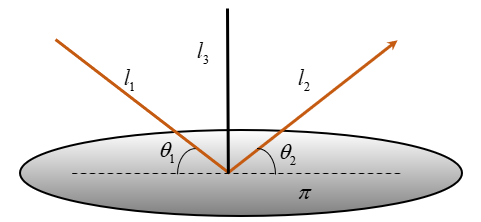
\includegraphics[width=0.8\textwidth]{vectors_mirror}
		\caption{Mirror}
	\end{figure}

	A student modelled the scenario such that the incident beam is ${l_1}$, the reflected beam is ${l_2}$ and the mirror is $\pi $, where $\pi $ contains the vectors ${\bf{i}} + {\bf{j}} + {\bf{k}}$, ${\bf{i}} - {\bf{j}}$ and $2{\bf{i}} + {\bf{j}} - {\bf{k}}$.

	\2 Find the equation of the plane $\pi $ in the form ${\bf{r}} \cdot {\bf{n}} = d$.\hfill[3]

	\2	Show that $P(1,3,2)$, the point of intersection between ${l_1}$ and ${l_2}$ lies on $\pi $.\hfill[1]

	\2	State the vector equation of ${l_3}$, the axis of reflection between ${l_1}$ and ${l_2}$.\hfill[1]

	\2	Given that $A(t,1,1)$ lies on ${l_1}$, where $t > 0$, find $t$ such that ${\theta _1} = {\theta _2} = \frac{\pi }{4}$.\hfill[4]	\\

	For the rest of the question, take $t = 4$.

	\2	Find the shortest distance from $A$ to $\pi $.\hfill[2]

	\2	Find the coordinates of $F$, the foot of perpendicular from $A$ to ${l_3}$. Hence, or otherwise, find the equation of ${l_2}$.\hfill[6]\\

	\newpage

	\1 A professional card stacker stacks two cards $P$ and $Q$ as follows:
	\begin{figure}[h]
		\centering
		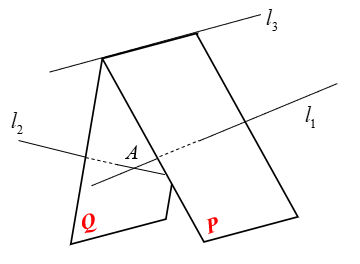
\includegraphics[width=0.5\textwidth]{vectors_tent}
		\caption{Card Stack}
	\end{figure}

	Mr Poh models the scenario such that the two cards are planes $P$ and $Q$, where the equation of plane $P$ is $P:{\bf{r}} \cdot \left( {\begin{array}{*{20}{c}}3\\{ - 1}\\1\end{array}} \right) = 1$, where line ${l_1}$ is a normal to plane $P$ that contains $A( - 3,3,2)$. Line ${l_2}$, a normal to plane $Q$, also contains point $A$ and is parallel to the vector $\left( {\begin{array}{*{20}{c}}3\\{ - 1}\\a\end{array}} \right)$ where $a < 0$. ${l_3}$ is the line of intersection between planes $P$ and $Q$.

	\2 Find the coordinates of $B$, the point of intersection between ${l_1}$ and plane $P$.\hfill[2]

	\2 Given that ${l_2}$ is obtaining by rotating ${l_1}$ ${\cos ^{ - 1}}\dfrac{9}{{11}}$ about point $A$, find $a$; Hence, find the vector equation of ${l_2}$.\hfill[4]

	\2 	The point of intersection between ${l_2}$ and plane $Q$ is point $B'$. Given that $\left| {\overrightarrow {AB} } \right| = \left| {\overrightarrow {AB'} } \right|$, find the position vector of $B'$ given that the $x$-coordinate of $B' < 0$.\hfill[3]

	\2	Find the equation of the plane $Q$ in the form ${\bf{r}} \cdot {\bf{n}} = d$.\hfill[2]

	\2	Find the vector equation of ${l_3}$.\hfill[2]\\

	The equation of plane $R$ is such that it reflects the image of plane $P$ to form plane $Q$.

	\2	Find the vector $\overrightarrow {AF} $, where $F$ is the foot of perpendicular from $A$ to ${l_3}$. \\
	Hence, find the equation of plane $R$ in the form ${\bf{r}} \cdot {\bf{n}} = d$.\hfill[5]

\end{outline}
\end{document}
